\clearpage
\section{Stakeholder analysis}
	
\subsection{Interested parties}
\textbf{Interested parties} are the groups of people who are being affected either negatively or positively by the problem in question. They have some influence over the development, as the trends and actions of these interested parties has to be taken into consideration by the development team and the people involved with the project. They don not necessarily take any direct action in the project.

\subsubsection{NASA}
The National Aeronautics and Space Administration, or more commonly known as NASA is a governmental agency in the United States, responsible for aerospace research and civilian space programs. Many manned- and unmanned missions to new planets require extensive research of that planet prior to the mission. It might even require sending exploratory rovers or satellites to examine the environment and to map out possible landing sites. Rovers are commonly used and equipped with similar technology that we are producing, as in all cases, the environment is unknown, external technologies, like GPS is not available and no maps are generated of these planets without previous research missions. 

\subsubsection{ESA}
The European Space Agency or simply ESA, is the European counter-part of NASA, governed by 22 member states, with the aim of space exploration and research. Similar interest applies to ESA as to NASA, therefore they can be classified as an \textit{Interested party} in our assessment.

\subsubsection{The Royal Danish Army}
The Royal Danish Army, or simply The Army, is the land warfare branch of the Danish Defense Forces, together with the Danish Home Guard. Their main tasks is to prevent conflicts and wars, through crisis management and co-operation with NATO and allied forces\cite{armytasks}. In case of a conflict or war, drones are commonly used to map out potential war sites before a planned attack or defense, and therefore The Army could potentially implement our mapping technology.

\subsubsection{The National Police}
Also known as \textit{Rigspolitet}\cite{Police}, The National Police is the national police force of Denmark, but also having authority over regions governed by The Kingdom of Denmark, the Faroe Islands and Greenland. As the nations main police force, it is part of their duty to avert any danger or possible terrorist attack in order to protect the population and public peace. As we identified dealing with terrorist attacks and hostage situations as a possible application for our technology, The National Police would be a potential user of such technology in these unfortunate events, assisting them with mapping a building where a kidnapping might take place or any other criminal offence, as an example.

\subsection{Actors}
We define \textbf{actors} as a subset of \textit{Interested parties}, who have any influence on the development of the project, either by financing it, providing knowledge or help the development of the project.

\subsubsection{Supervisors} 
The supervisors involved with this project are Akbar Hussain and Torben Rosenørn. Their involvement consists of giving directions regarding where to look for knowledge, having a general overview of the process and evaluating the end results of the project. They also provide valuable feedback and help through supervisor meetings to Group H103 during the duration of the project

\subsubsection{Department of Electronic Systems, AAU} 
The Department of Electronic Systems is one of the largest departments at Aalborg University with a total of more than 300 employees. The department is internationally recognized in particular for its contributions within Information and Communication Technology (ICT). As the project relates to a study line which is under the Electronics department, and therefore the tools, equipment and funding necessary for the project potentially could be funded by the department.
	
\subsection{Technology carriers}
We define \textbf{technology carriers} as a subset of \textit{Actors} who have influence to change the direction of the project, be involved with it or be a potential customer or partner in developing it further.

\subsubsection{Danish Explosive Ordnance Disposal squad} 
Also known as \textit{Ammunitionsrydningstjenesten} in Danish or \textit{EOD} for short, refers to the Danish bomb disposal squad\cite{EOD}. They are the one called in for emergency situations or bomb scares, where they use robots to map the area and find the possible suspicious items to investigate. The function of this squad is very crucial to the Danish Army, as these men and women need special training and education to work with these tools and technologies to ensure the public safety in these special cases. The interest that the Danish EOD squad would have in this project would be in regards of mapping technology and autonomous navigation in unknown terrains. Such technology could be used on rovers that bomb squads generally use for going in to building to find possible threats and to investigate it. This could mean they would have possible interest in the development, customization of the project to their needs and even financial interest. They are also considered as a potential users and carriers of this technology.

\subsubsection{Group H103}	
Group H103 is the group who develops the solution for this project. The group consists of:
\begin{itemize}
	\item Antal János Monori
	\item Emil Már Einarsson
	\item Gustavo Smidth Buschle
	\item Thomas Thuesen Enevoldsen
\end{itemize}

\subsection{Summary}
\begin{table}[H]
	\begin{tabular}{ | p{5cm} | l | p{5cm} |}
	   	\hline
	   	\bfseries Name of stakeholder & \bfseries Type & \bfseries Role \\ \hline
	   	Group H103 & Technology carriers & Developing the project \\ \hline
	   	Danish Explosive Ordnance Disposal squad & Technology carriers & Knowledge sharing and potential partner/client  \\ \hline
	   	Electronics dept., AAU & Actors & Funding\\ \hline
	   	Supervisors & Actors & Knowledge sharing and assistance \\ \hline
 	   	NASA & Interested parties & Potential partner/client \\ \hline
 	   	ESA & Interested parties & Potential partner/client \\ \hline
 	   	The Royal Danish Army & Interested parties & Potential partner/client \\ \hline
 	   	The National Police & Interested parties & Potential partner/client \\
	   	\hline
	\end{tabular}
	\caption{Stakeholder table}
	\label{table:stakeholdertable}
\end{table}

The table above contains the names of the different people involved with or interested in the project, with the type, role and impact of their involvement specified. The type of the stakeholder represents a level of involvement within the project, meanwhile the role represents a more concrete function.

\begin{figure}[H]
	\centering
	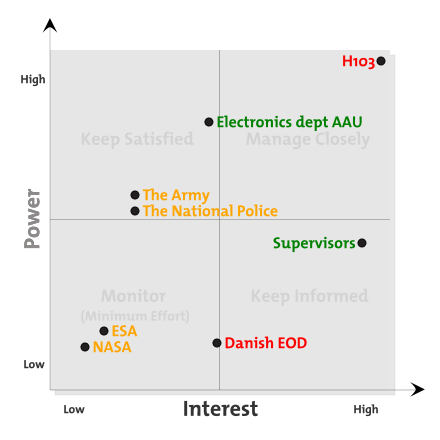
\includegraphics[scale=.6]{images/stakeholderanalysis.png}
	\caption{Stakeholder analysis diagram}
	\label{fig:stakeholder}
\end{figure}

The following chart showcases how do we categorize our stakeholders on the Power/Interest grid, used commonly for stakeholder analysis.
The different colors used for distinguishing between the three types of stakeholders we identified: orange for \textit{interested parties}, green for \textit{actors} and red for \textit{technology carriers}.
The for sections can be defined as:
\begin{itemize}
	\item \textbf{High power, interested people:} these are the people you must fully engage and make the greatest efforts to satisfy.
	\item \textbf{High power, less interested people:} put enough work in with these people to keep them satisfied, but not so much that they become bored with your message.
	\item \textbf{Low power, interested people:} keep these people adequately informed, and talk to them to ensure that no major issues are arising. These people can often be very helpful with the detail of your project.
	\item \textbf{Low power, less interested people:} again, monitor these people, but do not bore them with excessive communication.
\end{itemize}